\subsection{An R and \protect\pbdR View of Parallel Hardware and Software}
%\makesubcontentsslidessec

\begin{frame}{R Interfaces to Low-Level Native Tools}
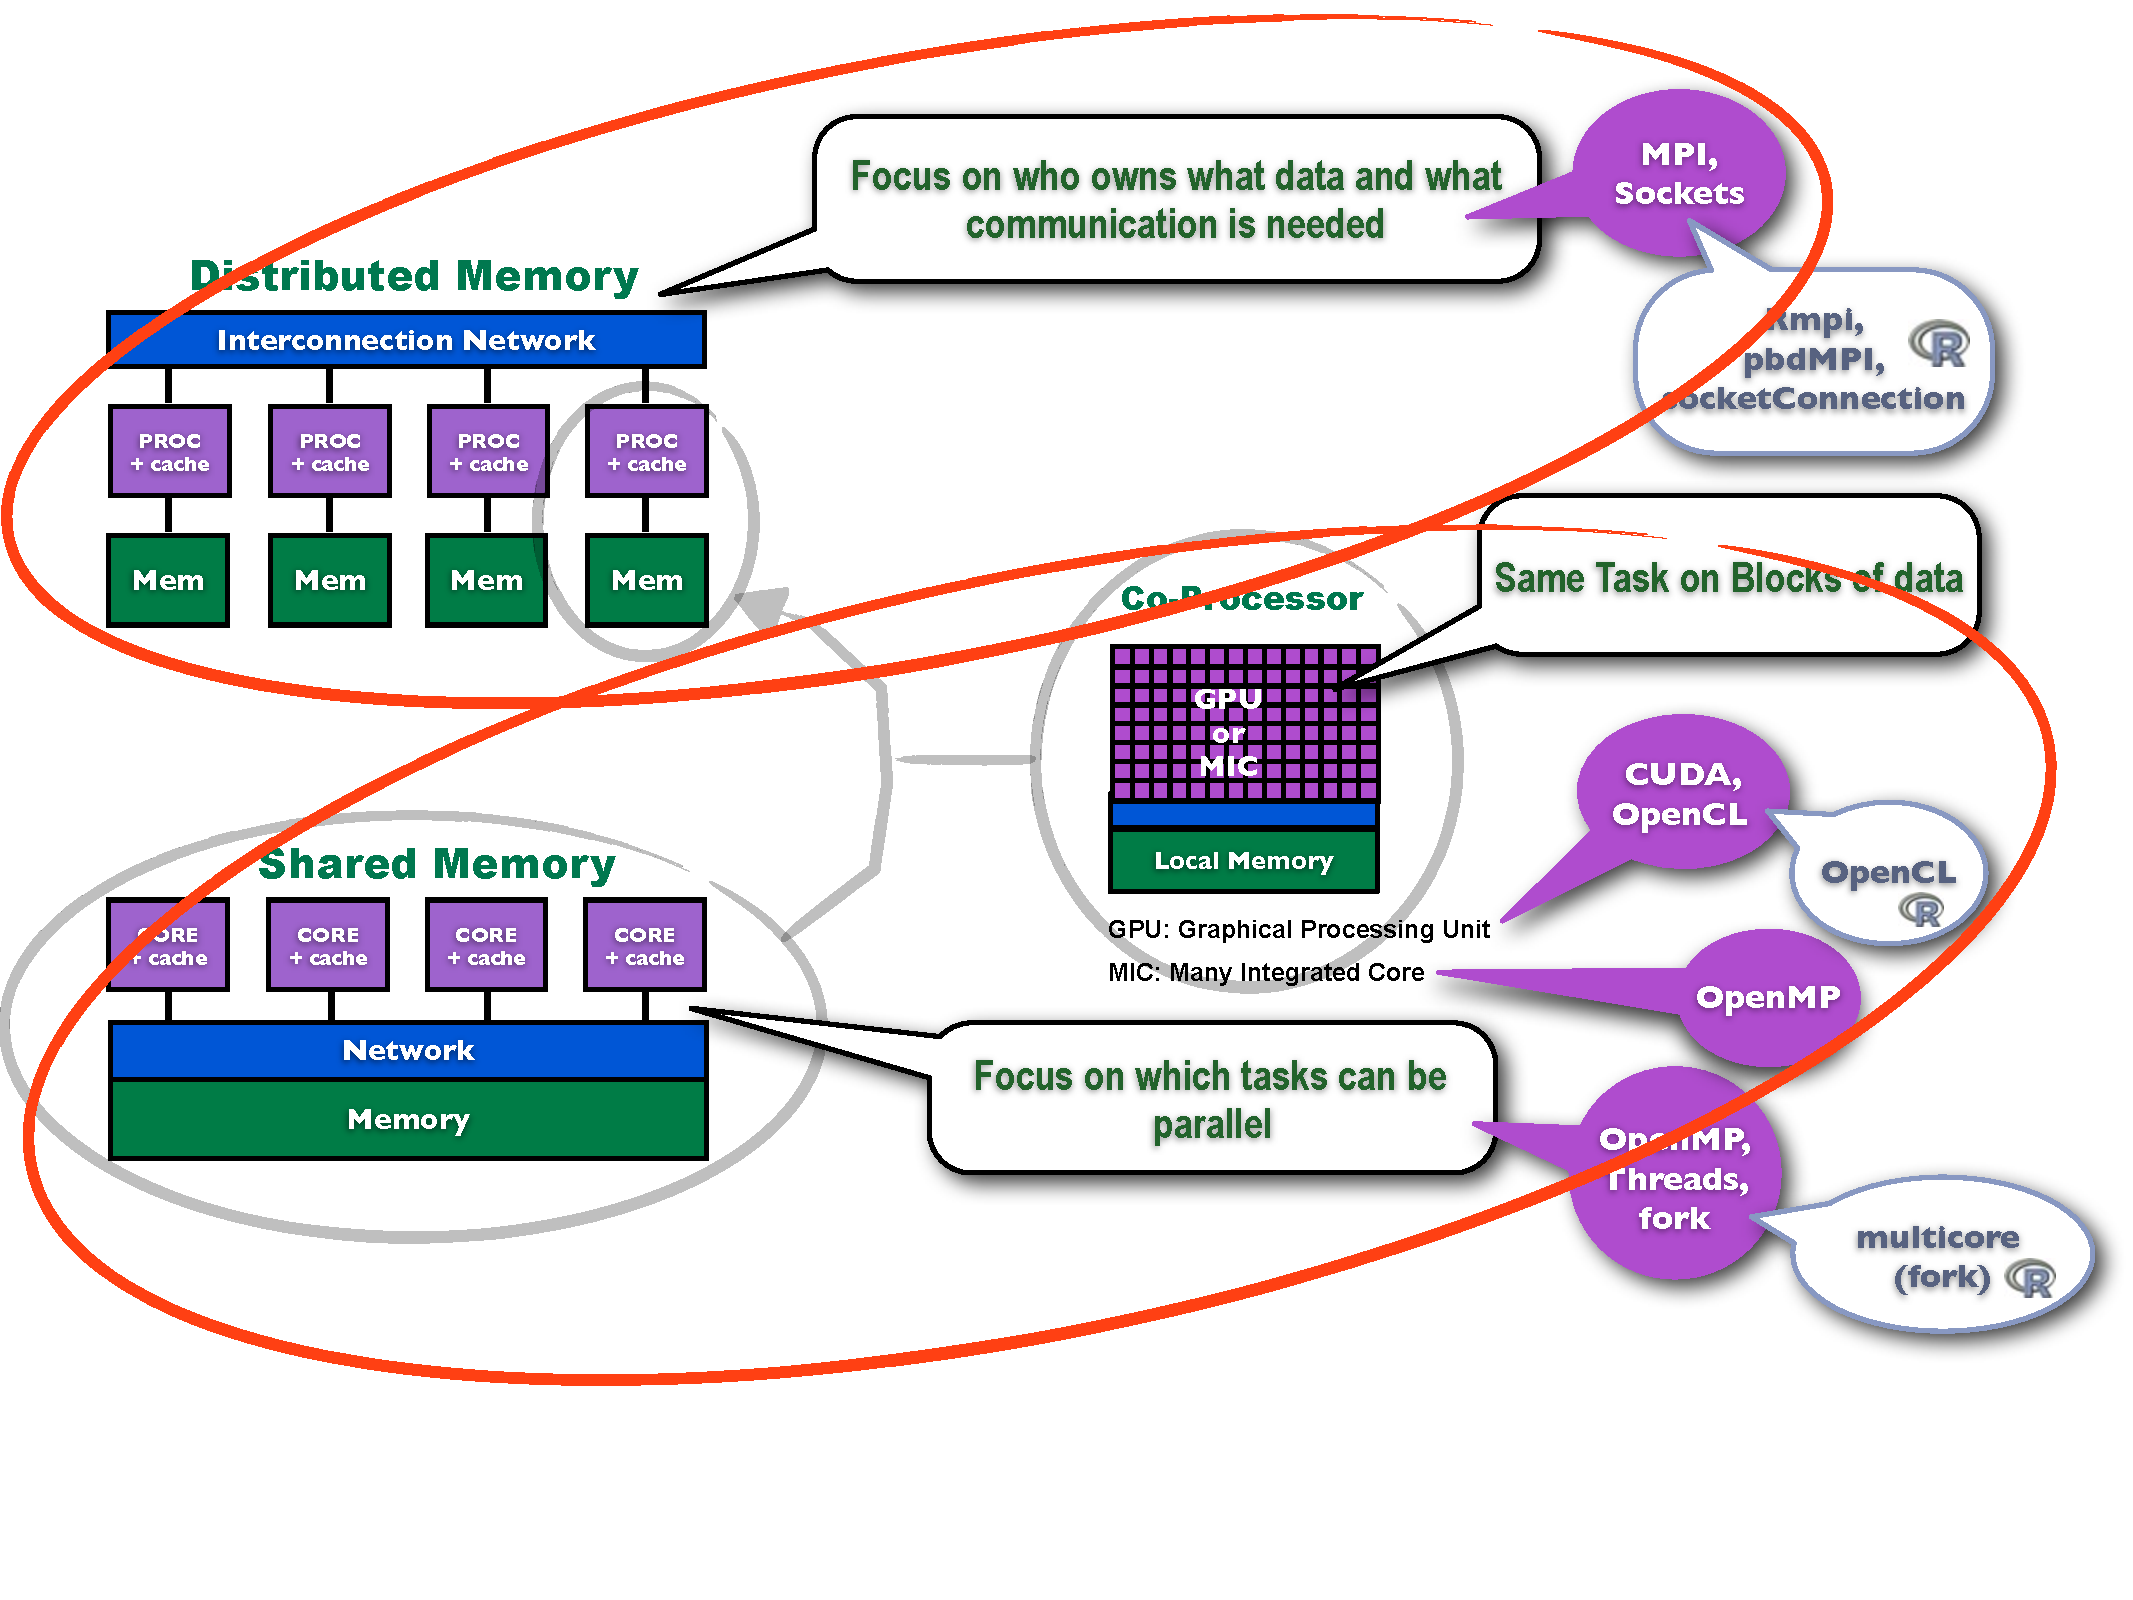
\includegraphics[width=1.30\textheight]
{../common/pics/hardware/ParallelHardware10.pdf}
\end{frame}

\begin{frame}{Big Data and Little Data}
\begin{minipage}{10cm}
  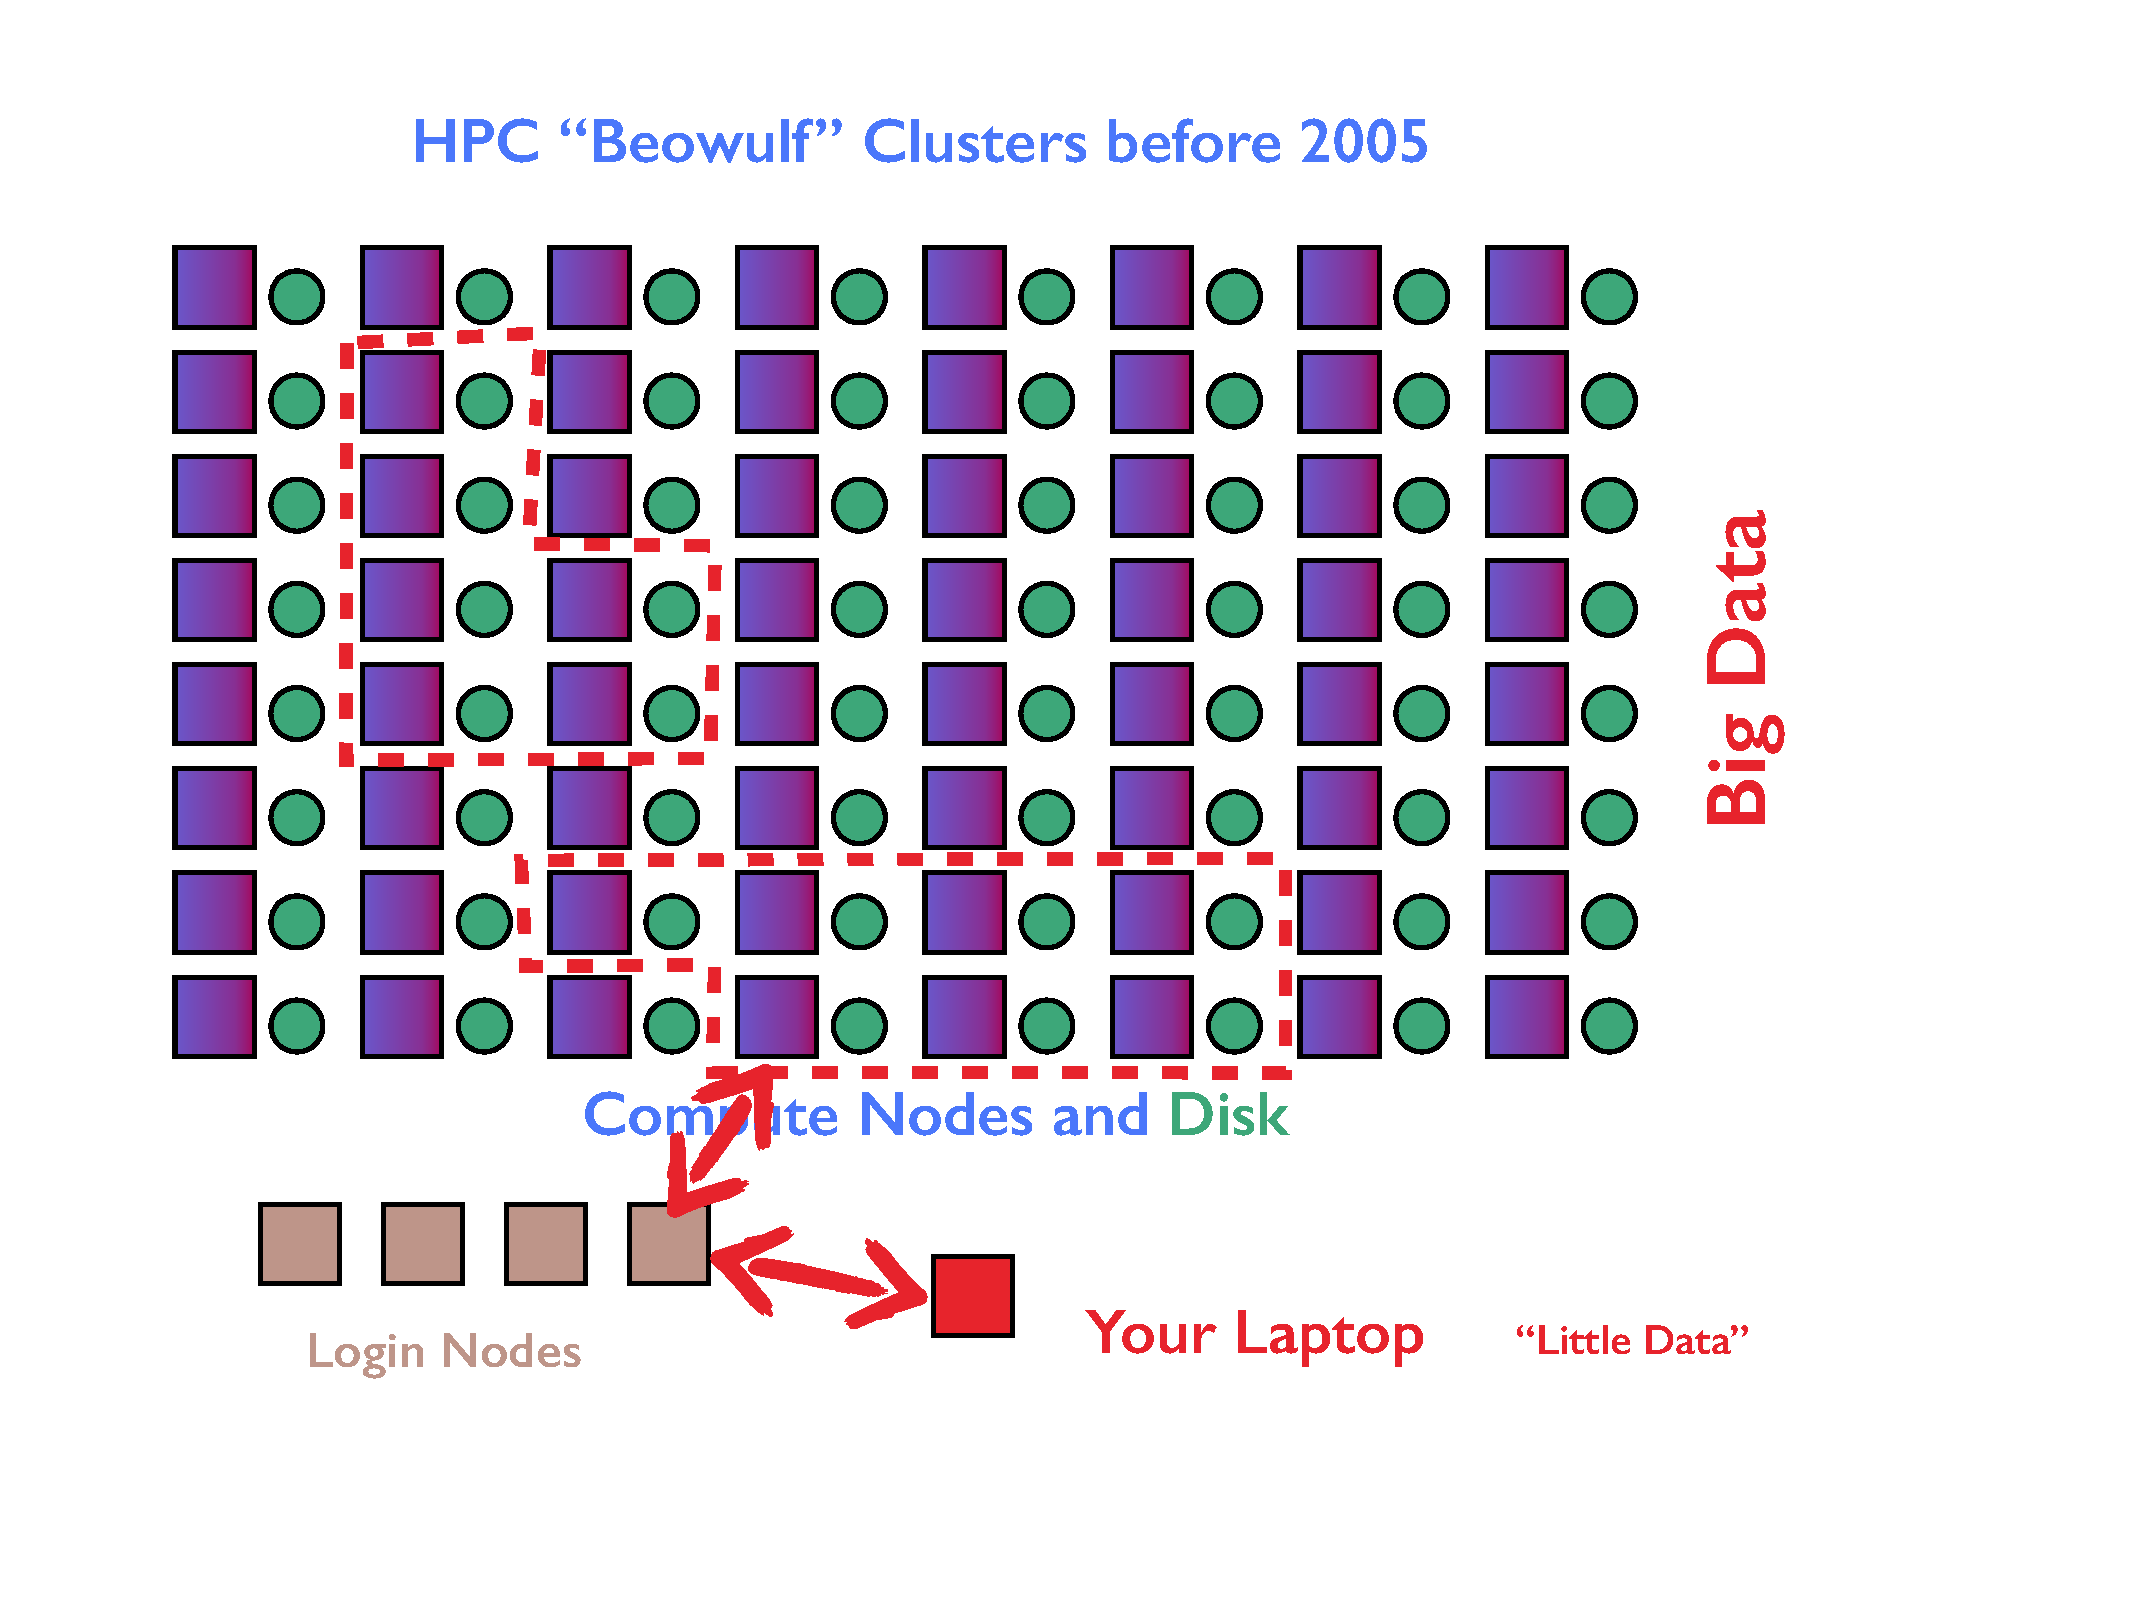
\includegraphics[width=1.2\textheight]
  {../common/pics/hardware/ParallelHardware22.pdf}\hfill
\end{minipage}
\begin{minipage}{5cm}\small
  \begin{block}{Analysis Workflow}\pause
    \begin{itemize}[<+-|alert@+>]
    \item Get Big Data
      \begin{itemize}
      \item Parallel data reader
      \item Parallel data generator
      \end{itemize}
    \item Write analysis script
    \item Graphics to display results
    \item Profile and optimize code
    \end{itemize}
  \end{block}
\end{minipage}
\end{frame}

\begin{frame}{R and \pbdR Interfaces to Libraries: Harness 30+ Years of
    HPC Research}
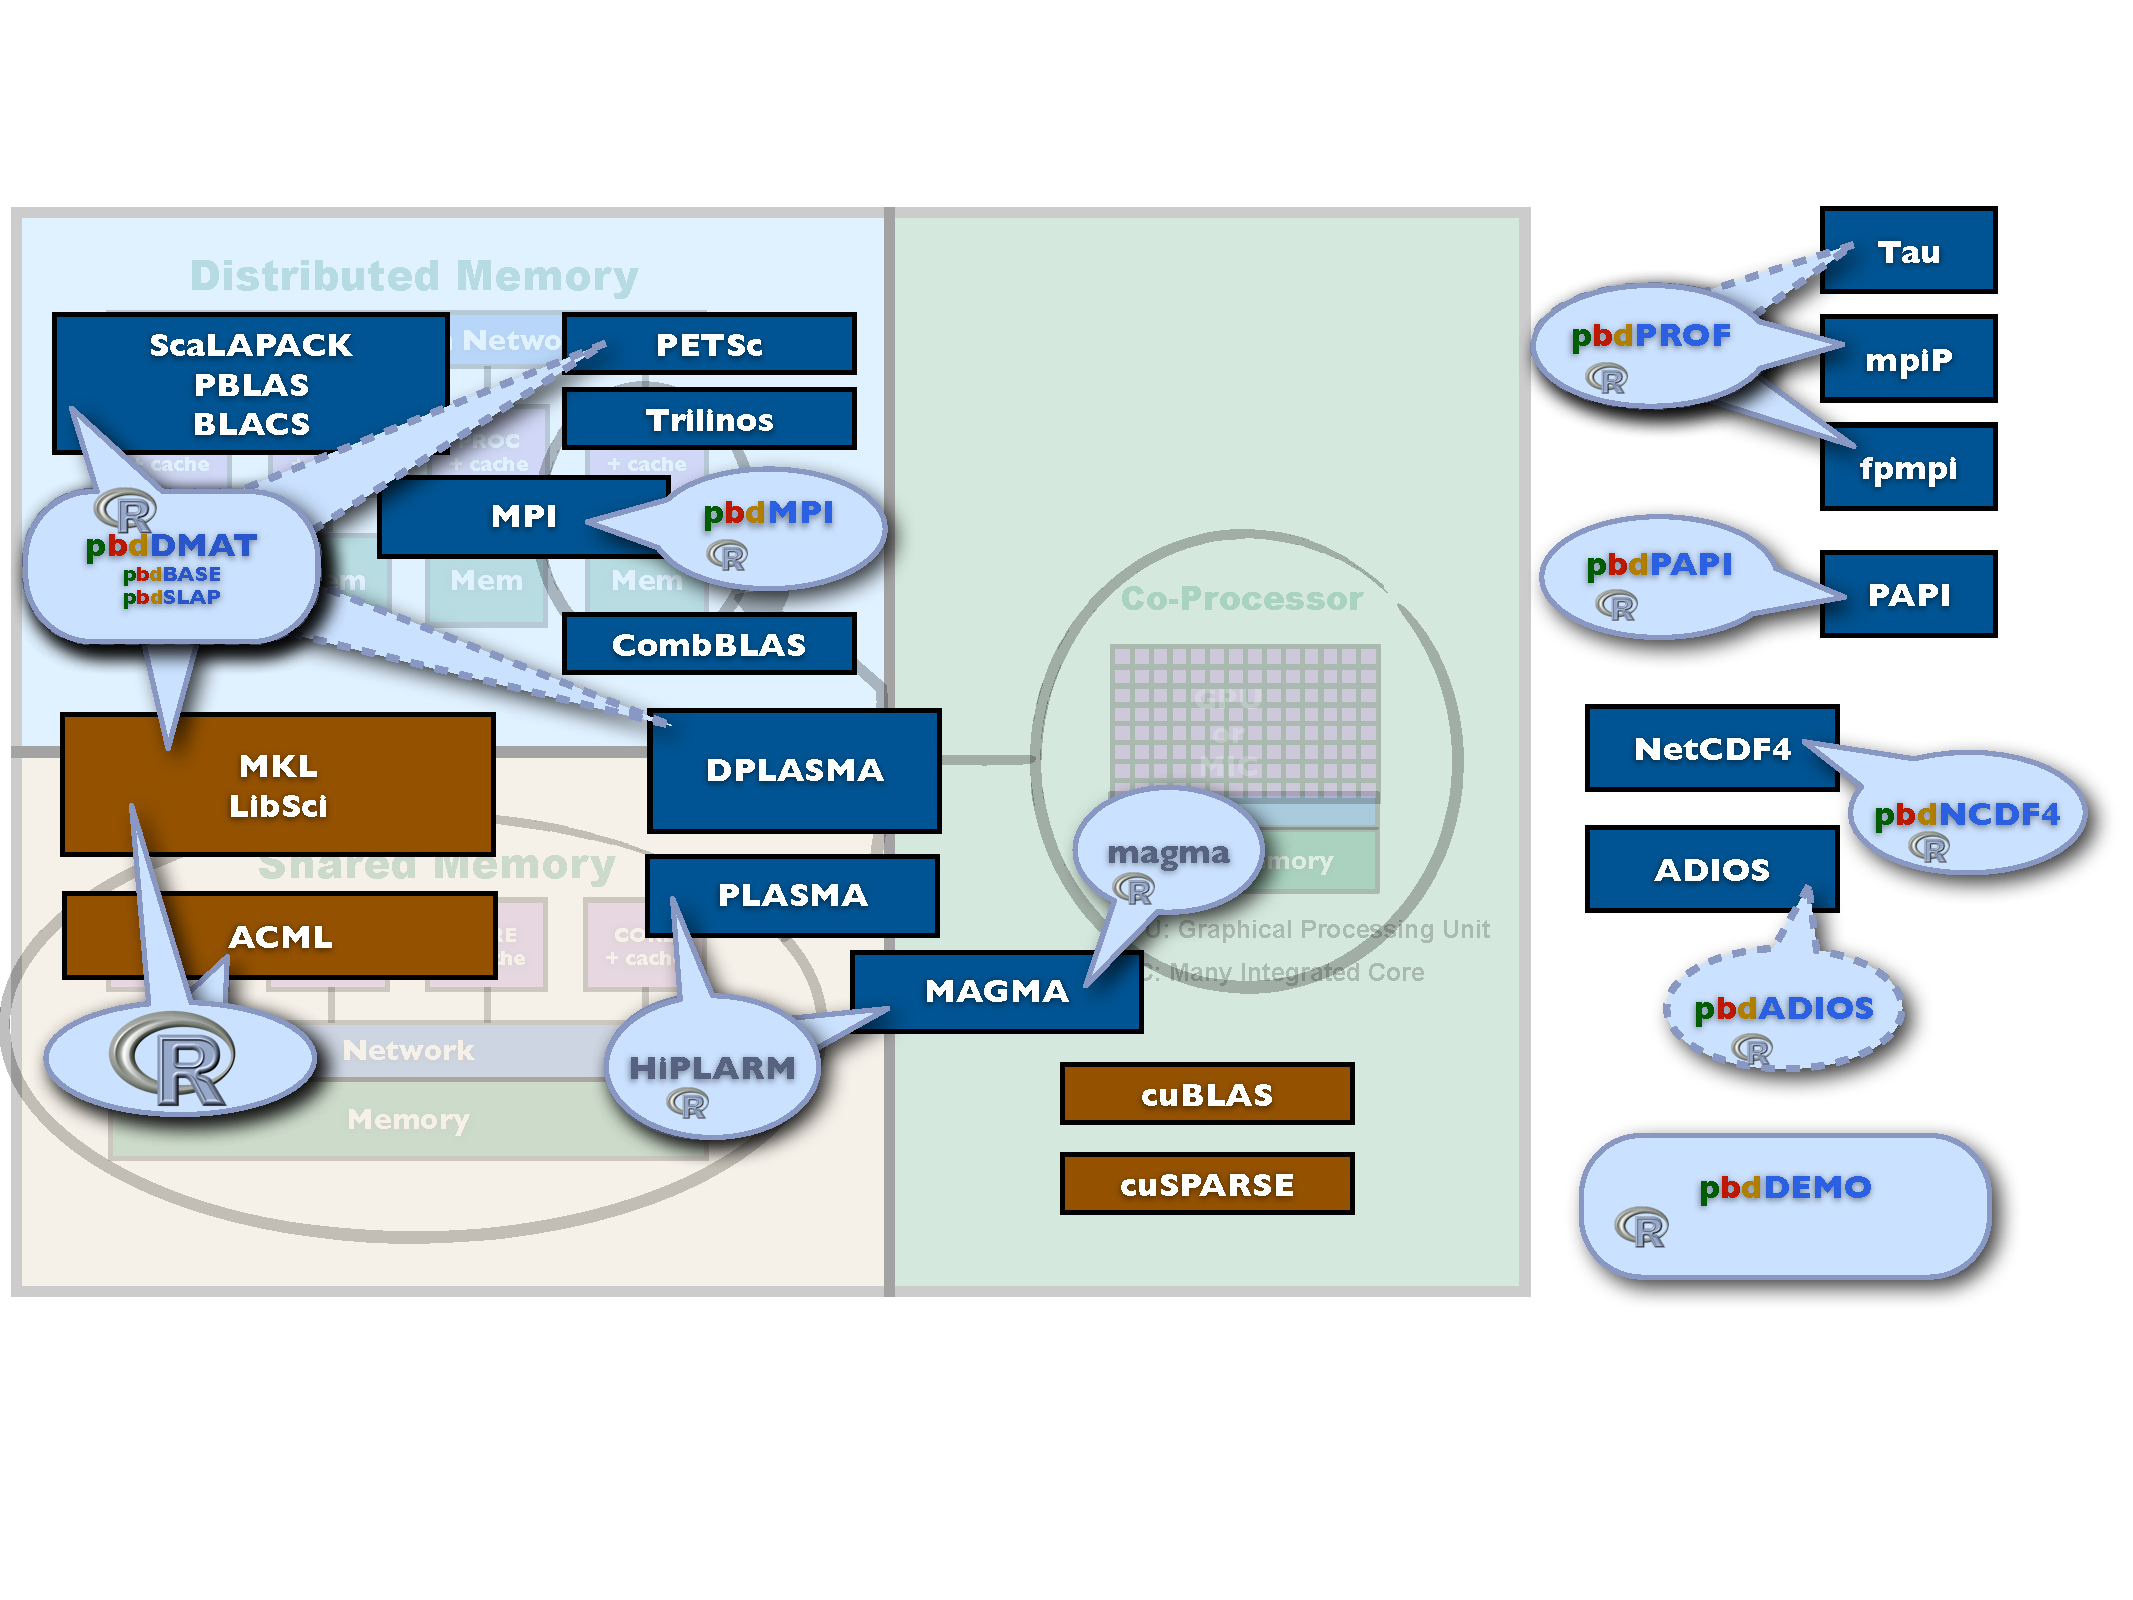
\includegraphics[width=1.35\textheight]
{../common/pics/hardware/ParallelHardware14.pdf}
\end{frame}

\begin{frame}{Hadoop: Can use HDFS but replace rest with HPC libraries}
\begin{minipage}{10cm}
  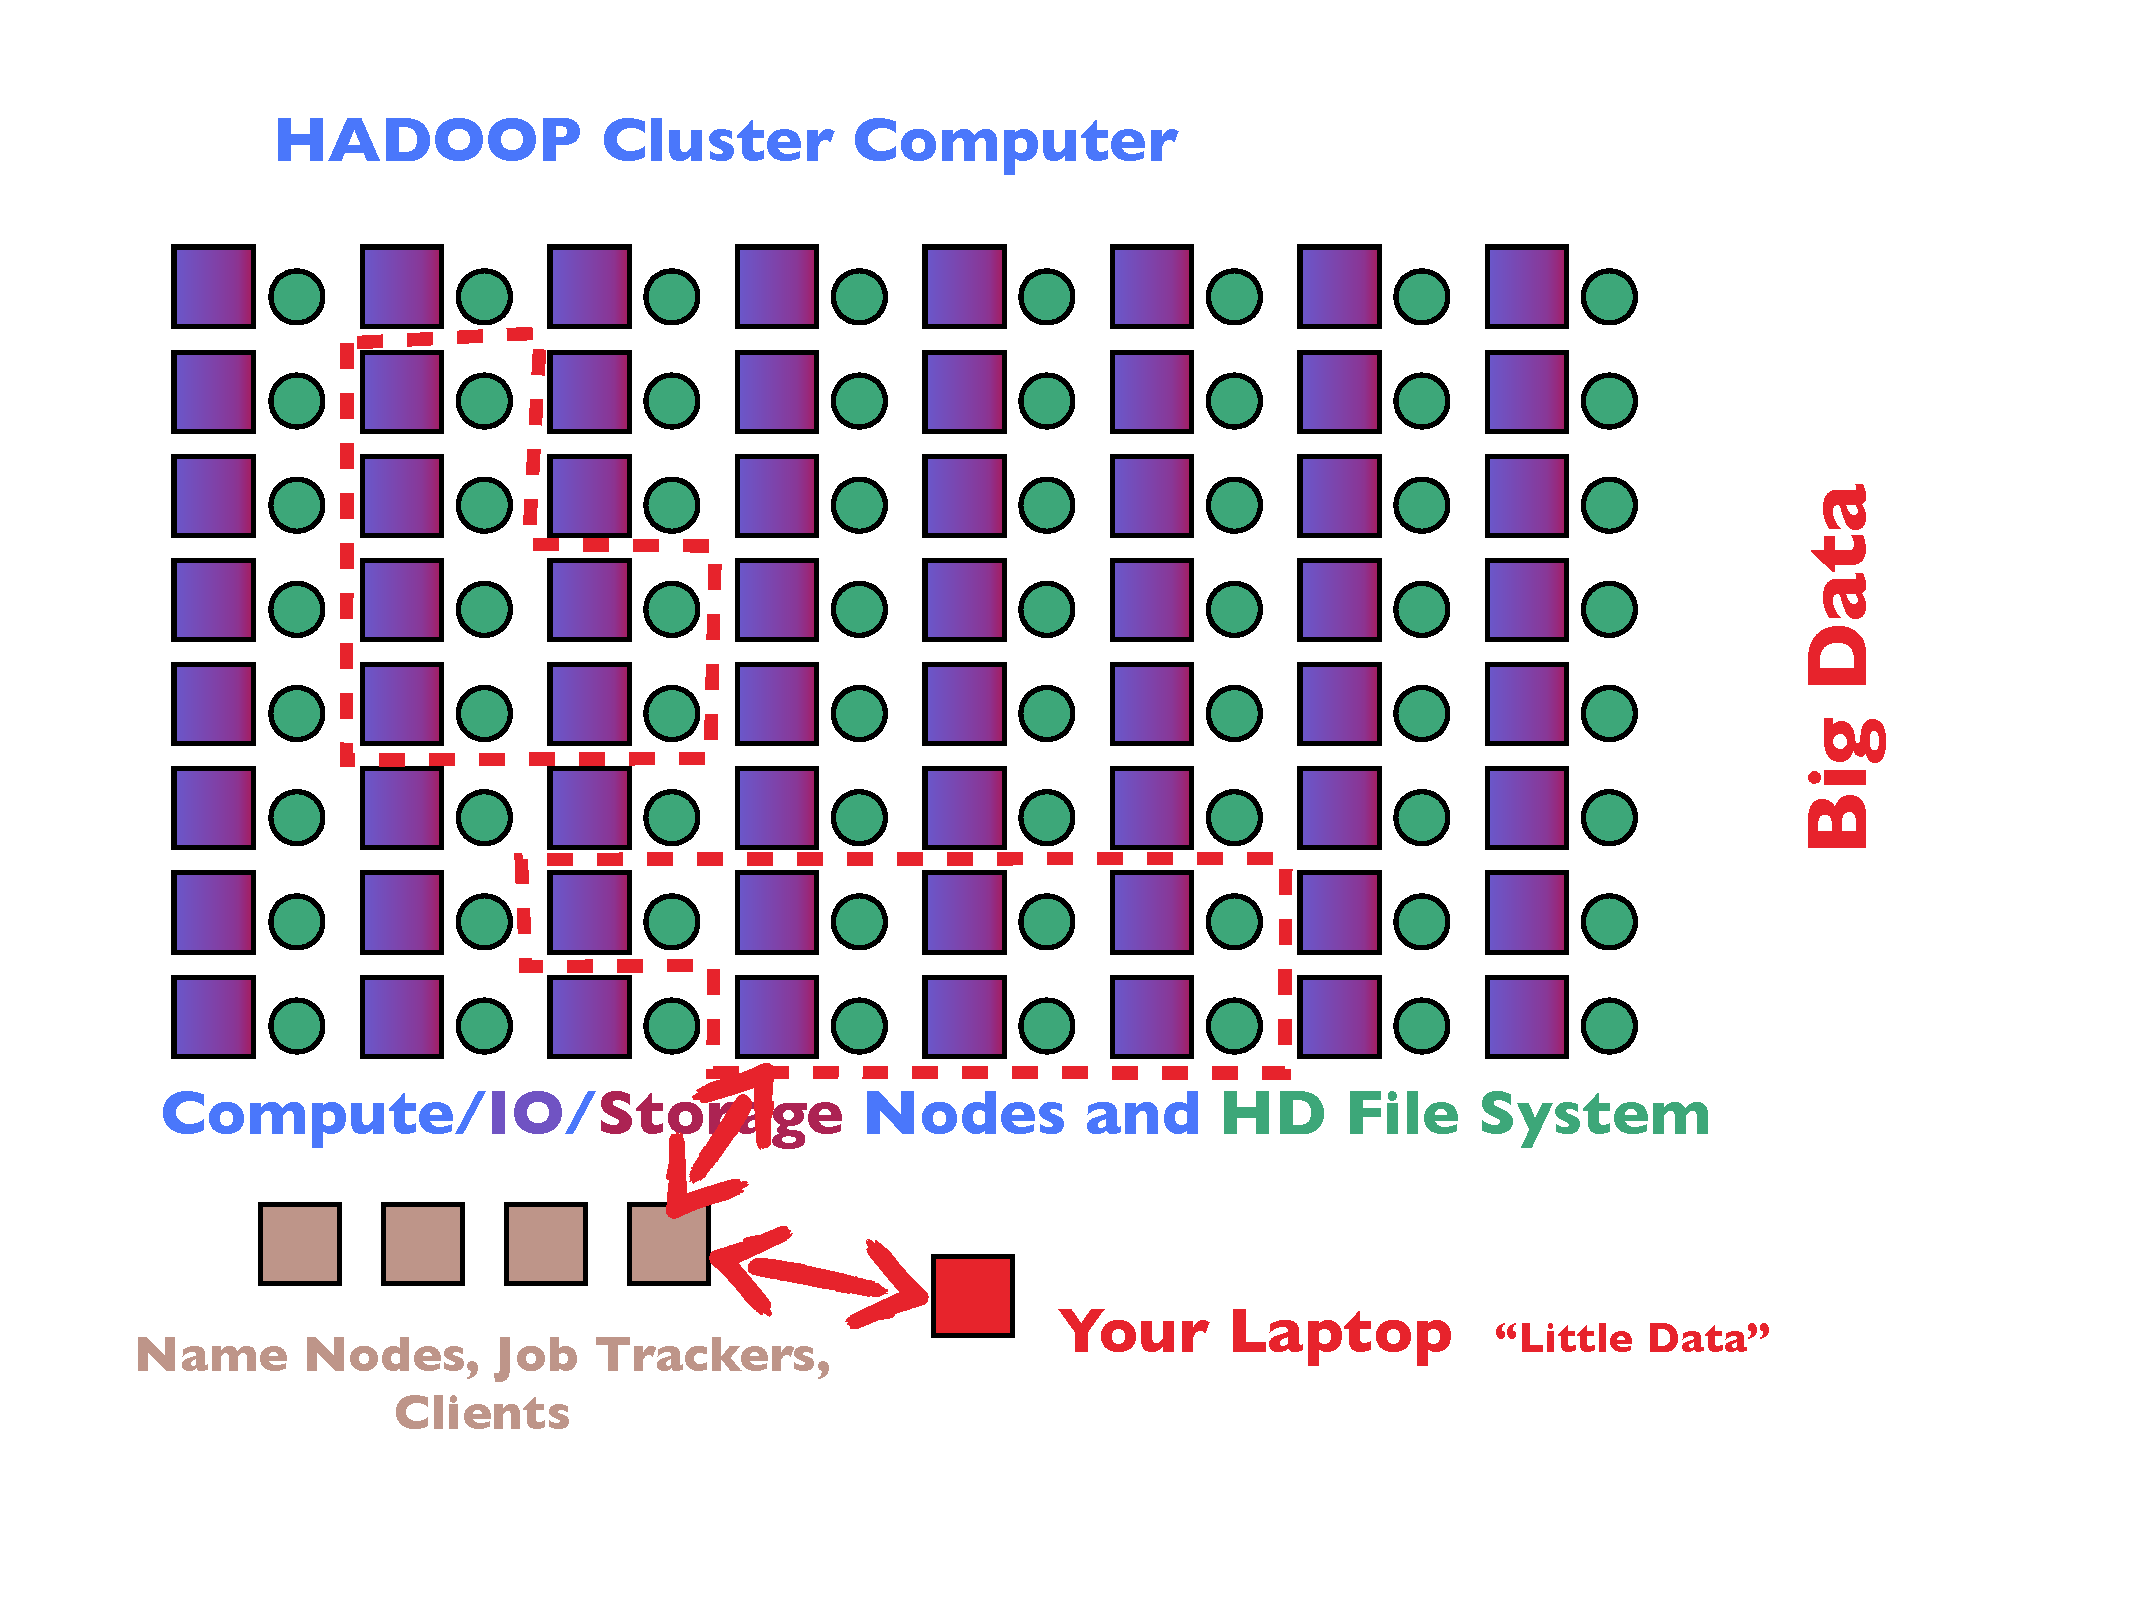
\includegraphics[width=1.25\textheight]
  {../common/pics/hardware/ParallelHardware23.pdf}
\end{minipage}
\begin{minipage}{5cm}\small
  \begin{block}{Three Hadoop components}\pause
    \begin{itemize}[<+-|alert@+>]
    \item File system: HDFS
    \item Resource manager: Yarn
    \item Algorithm limitation: Map Reduce, Manager+Workers
    \end{itemize}
  \end{block}
\end{minipage}
\end{frame}

\begin{frame}{R and \pbdR Interfaces to Libraries: ``Standing on the Shoulders of
  Giants''}
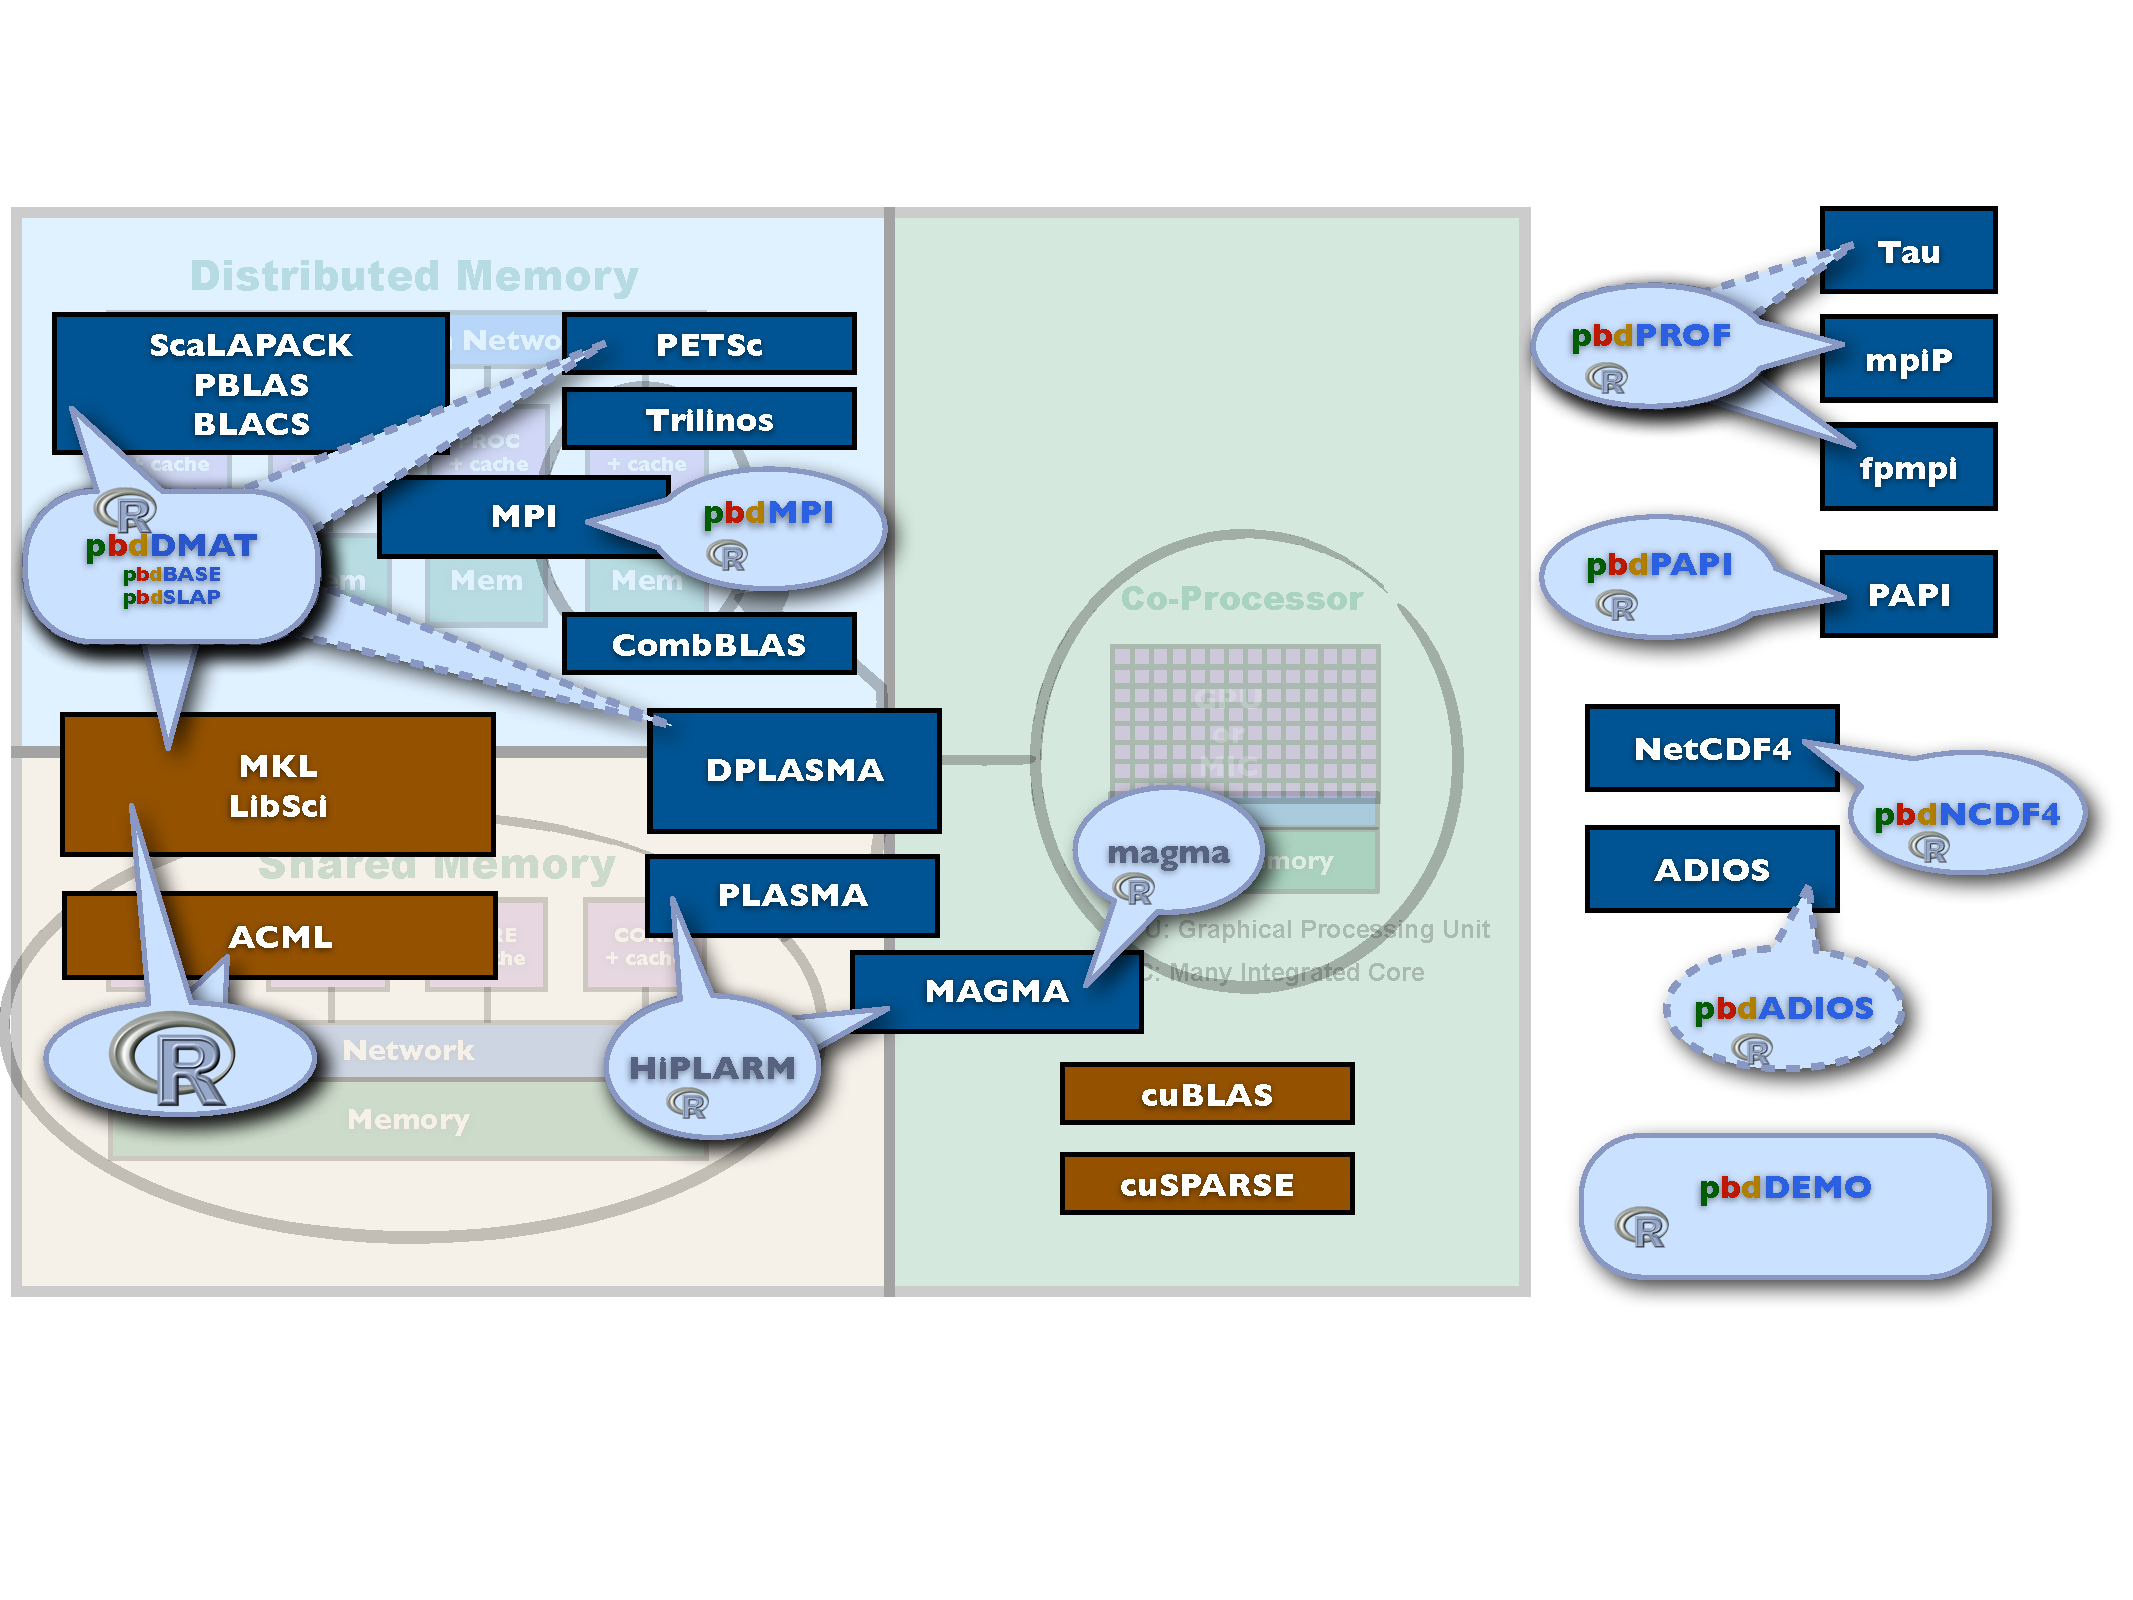
\includegraphics[width=1.35\textheight]
{../common/pics/hardware/ParallelHardware14.pdf}
\end{frame}

%\begin{frame}{Low level R Interfaces to Native Tools}
%\includegraphics[width=0.95\textheight]
%{../common/pics/hardware/ParallelHardware22.pdf}
%\includegraphics[width=0.95\textheight]
%{../common/pics/hardware/ParallelHardware23.pdf}
%\end{frame}

